% !TeX spellcheck = en_US

\chapter{Introduction}
\section{Technical Background - PNF / AV}
tbd

\section{Architecture}
\autoref{fig:introduction:architecture_overview} shows an overview of the architecture. Note, that this diagram shows a combination of the learning and the prediction architecture. Step 2, which is loading the satellite imagery from Microsoft Bing is only required in the learning phase, that is for the generation of the training data, which is required to train the neural network.

\begin{figure}[H]
    \centering
	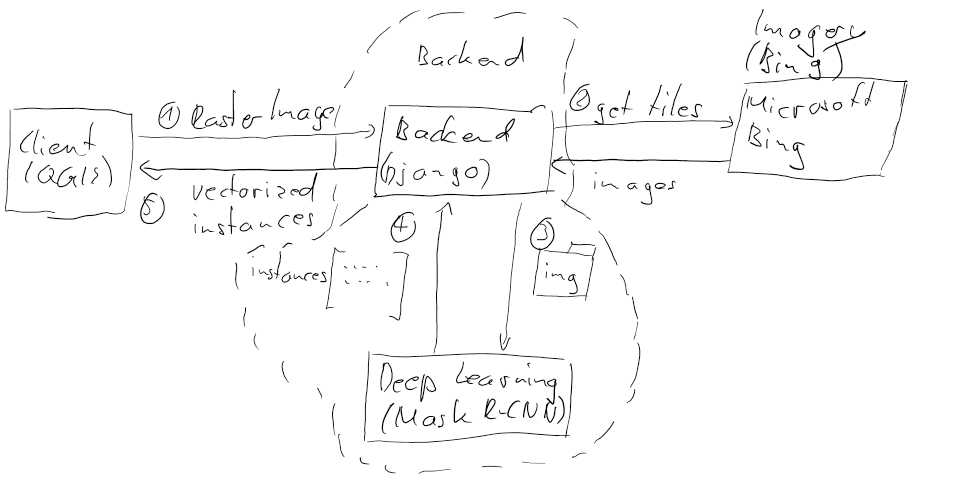
\includegraphics[width=0.9\linewidth]{chapters/introduction/images/overview.png}
	\caption{Architecture overview}
	\label{fig:introduction:architecture_overview}
\end{figure}

\autoref{fig:introduction:learning_phase} shows the data flow during the training of the neural network. For this step, satellite imagery from Microsoft Bing maps as well as OpenStreetMap (OSM) data is used. The satellite imagery is downloaded tile per tile for a predefined boundingn box and zoom-level and at the same time, binary images are created from the OSM data, which represent the ground truth. To simplify this step and make it available to the public, a tool called Airtiler \cite{airtiler} has been created and published.

\begin{figure}[H]
    \centering
	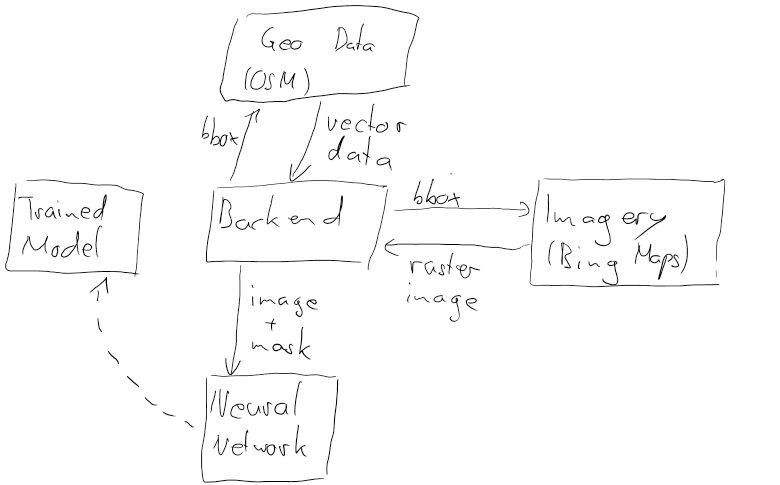
\includegraphics[width=0.9\linewidth]{chapters/introduction/images/learning_phase.png}
	\caption{Learning phase}
	\label{fig:introduction:learning_phase}
\end{figure}

As soon as the training is completed, the prediction can be done. For this thesis, this has been split into two phases. \autoref{fig:introduction:prediction_phase1} shows the data flow of phase 1, which passes the current extent as base64 encoded image data as well as the bounding box of the current QGIS extent to the configured backend webserver. The pretrained neural network is then used, to predict all instances on the current image. In the next step, the predicted instances are georeferenced using the boundingbox information that was sent to the backend at the beginning of the prediction phase. Finally, the georeferenced instances are sent back to the frontend client (the QGIS plugin), which then visualizes the data on a new layer in QGIS.

\begin{figure}[H]
    \centering
	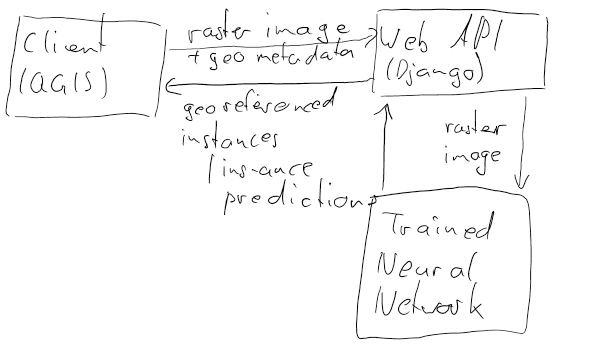
\includegraphics[width=0.9\linewidth]{chapters/introduction/images/inference_phase1.png}
	\caption{Prediction phase 1}
	\label{fig:introduction:prediction_phase1}
\end{figure}

\begin{figure}[H]
    \centering
	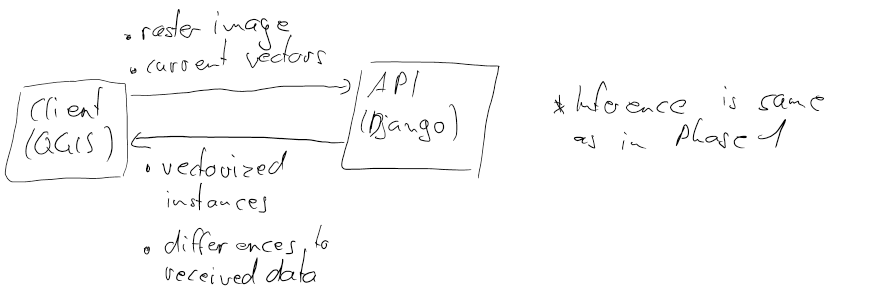
\includegraphics[width=0.9\linewidth]{chapters/introduction/images/inference_phase2.png}
	\caption{Prediction phase 2}
	\label{fig:introduction:prediction_phase2}
\end{figure}



